% !TEX TS-program = pdflatex
% !TeX program = pdflatex
% !TEX encoding = UTF-8
% !TEX spellcheck = fr

\documentclass{beamer}
%\usepackage{fullpage}
%\usepackage[left=2.8cm,right=2.2cm,top=2 cm,bottom=2 cm]{geometry}
\setbeamersize{text margin left=10pt,text margin right=10pt}
\usepackage{amsmath,amssymb} 
\usepackage[T1]{fontenc}
\usepackage[utf8]{inputenc}
\usepackage[english,french]{babel}
\usepackage{txfonts}
\usepackage[]{graphicx}
\usepackage{multirow}
\usepackage{hyperref}
\usepackage{listings}
\usepackage{wrapfig}


\hypersetup{
	colorlinks,
	urlcolor = blue
}

%\renewcommand{\baselinestretch}{1.5}

\def\supit#1{\raisebox{0.8ex}{\small\it #1}\hspace{0.05em}}

\makeatletter
\newcommand\mysphere{%
	\parbox[t]{10pt}{\raisebox{0.2pt}{\beamer@usesphere{item projected}{bigsphere}}}}
\makeatother

\AtBeginSection{%
	\begin{frame}
		\sectionpage
	\end{frame}
}

\newcommand{\rottext}[2]{%
	\rotatebox{90}{%
	\begin{minipage}{#1}%
		\raggedleft#2%
	\end{minipage}%
	}%
}

\usepackage{longtable}
\usepackage{tabu}


\title[BWEB: 01- RI et Gmail] %
{Bureautique et Web \\Chapitre 02: Recherche d'information et messagerie} 
\institute{ %
École  nationale Supérieure d'Informatique (ESI, ex. INI), Algérie
}
\author[ \textbf{\footnotesize  \insertframenumber/\inserttotalframenumber} \hspace*{1cm} ESI - ARIES Abdelkrime (2019-2020)] %
{ARIES Abdelkrime}
%\titlegraphic{
\includegraphics[height=1cm]{../img/esi-logo.png}%\hspace*{4.75cm}~


\date{Année unniversitaire: 2019/2020} %\today

\usetheme{Warsaw} % Antibes Boadilla Warsaw

\beamertemplatenavigationsymbolsempty

%\setbeamertemplate{headline}{}


\begin{document}
	
	\newcolumntype{L}[2]{%
		>{\vbox to #2\bgroup\vfill\flushleft}%
		p{#1}%
		<{\egroup}} 

\begin{frame}[plain]
	\maketitle
\end{frame}

%===================================================================================
\section{Recherche d'information}
%===================================================================================

\begin{frame}
\frametitle{Recherche d'information}

%Pour préparer un rapport ou une présentation: 
%\begin{itemize}
%	\item Cerner le sujet 
%	\item Localiser l'information 
%	\item Collecter les informations 
%	\item Traiter l'information 
%	\item Restituer l'information 
%	\item Rédiger le travail
%\end{itemize} 

\includegraphics[height=.9\textheight]{..//img/Bweb02-ri-gmail/etapes-rapport.pdf}


\end{frame}

\subtitle{Localiser l'information sur le web}

\begin{frame}
\frametitle{Recherche d'information}
\framesubtitle{Localiser l'information sur le web}

Afin de localiser l'information sur le web: 
\begin{itemize}
	\item Exploration des ressources 
	\begin{itemize}
		\item On doit savoir exactement les sites web utiles pour son sujet 
		\item On suit les liens des sites similaires
	\end{itemize}
	\item Recherche par mots clés
	\begin{itemize}
		\item On définit des mots clés relatifs a son sujet  
		\item On utilise des moteurs de recherche pour trouver les ressources nécessaire
	\end{itemize}
\end{itemize} 

\end{frame}


\begin{frame}
\frametitle{Recherche d'information: Localiser l'information sur le web}
\framesubtitle{Exploration des ressources}

\begin{itemize}
	\item Avantages
	\begin{itemize}
		\item Un site spécifique à un domaine ne contient que des informations utiles (pour un sujet de ce domaine) 
		\item Sauver le temps de recherche et de sélections des sites 
	\end{itemize}
	\item Inconvénients
	\begin{itemize}
		\item On doit être familier avec les sites de chaque domaine 
		\item Les liens peuvent êtres obsolètes (ne marchent plus)
	\end{itemize}
\end{itemize} 

\end{frame}


\begin{frame}
\frametitle{Recherche d'information: Localiser l'information sur le web}
\framesubtitle{Recherche par mots clés}

\begin{itemize}
	\item Avantages
	\begin{itemize}
		\item Rapide et n'exige pas une connaissance des ressources
		\item Fournit beaucoup de résultats: diversité de ressources
	\end{itemize}
	\item Inconvénients
	\begin{itemize}
		\item Dépend des mots clés introduits; s'ils ne sont pas bons, les résultats le sont aussi
		\item Fournit des résultats inutiles: trouver les bonnes ressources peut prendre du temps
	\end{itemize}
\end{itemize} 

\end{frame}


\subsection{Moteurs de recherche}

\begin{frame}
\frametitle{Recherche d'information}
\framesubtitle{Moteurs de recherche}

\begin{definition}
	Un moteur de recherche est une application informatique permettant de localiser des ressources en utilisant des mots clés.
\end{definition}

Mesurer l'efficacité d'un moteur de recherche:
\begin{itemize}
	\item Pertinence de résultats: parmi les résultats fournis par le moteur, le nombre de résultats utiles à l'utilisateur doit être grand. Un métrique pour mesurer la qualité est \textcolor{red}{Recouvrement}.
	{\scriptsize \[ Recouvrement = \frac{nombre\ des\ résultats\ utiles\ parmi\ ceux\ fournis\ par\ le\ moteur}{nombre\ total\ des\ résultats\ fournis\ par\ le\ moteur} \]}
	\item Temps de réponse: Un moteur de recherche doit être rapide
\end{itemize}

\end{frame}

\begin{frame}
\frametitle{Recherche d'information: Moteurs de recherche}
\framesubtitle{Types des moteurs de recherche}

Un moteur de recherche peut être:
\begin{itemize}
	\item Selon le fonctionnement
	\begin{itemize}
		\item annuaire
		\item explorateur
		\item méta-moteur
	\end{itemize}

	\item Selon la spécialité
	\begin{itemize}
		\item générique
		\item académique
		\item de bureau 
		\item de développement
		\item ...
	\end{itemize}
\end{itemize} 

\end{frame}


\begin{frame}
\frametitle{Recherche d'information: Moteurs de recherche}
\framesubtitle{Types des moteurs de recherche selon le fonctionnement}


\begin{itemize}
	\item Annuaires
	\begin{itemize}
		\item Les liens sont introduit manuellement, et validés par un administrateur
		\item La recherche se fait sur la description (manuelle) de la ressource 
		\item Les ressources sont organisées en catégories 
	\end{itemize}
	
	\item Explorateurs
	\begin{itemize}
		\item Les liens sont introduits automatiquement en utilisant l'exploration 
		\item La recherche se fait sur le contenu des ressources
		\item Les résultats sont organisées selon la pertinence à la requête (ou selon d'autres critères)
	\end{itemize}

	\item Méta-moteurs
	\begin{itemize}
		\item Ne sauvegardent pas les liens 
		\item La recherche se fait en utilisant d'autres moteurs de recherche
		\item Les résultats sont organisées selon la pertinence à la requête (ou selon d'autres critères)
	\end{itemize}
\end{itemize} 

\end{frame}


\begin{frame}
\frametitle{Recherche d'information: Moteurs de recherche}
\framesubtitle{Quelque moteurs de recherche web (génériques)}

\def\arraystretch{0}

\begin{tabular}{L{.3\textwidth}{.8cm}cp{.6\textwidth}}%p{.3\textwidth}
	
	\hline
	
	
\includegraphics[height=.8cm]{..//img/Bweb02-ri-gmail/google-logo.png} &
	& 
	\url{https://www.google.com/}  \\
	
	\hline
	
	
\includegraphics[height=.8cm]{..//img/Bweb02-ri-gmail/bing-logo.png} &
	& 
	\url{https://www.bing.com/} \\
	
	\hline
	
	
\includegraphics[height=.4cm]{..//img/Bweb02-ri-gmail/yahoo-logo.png} & 
	& 
	\url{https://search.yahoo.com/} \\
	
	\hline
	
	
\includegraphics[height=.8cm]{..//img/Bweb02-ri-gmail/baidu-logo.png} & 
	& 
	\url{https://www.baidu.com/} \\
	
	\hline
	
	
\includegraphics[height=.8cm]{..//img/Bweb02-ri-gmail/yandex-logo.png} & 
	& 
	\url{https://yandex.com/} \\
	
	\hline
	
\end{tabular}

%\begin{itemize}
%	\item Google
%	\item Bing 
%	\item Yahoo
%	\item DuckDuckGo
%\end{itemize}

\end{frame}


\begin{frame}
\frametitle{Recherche d'information: Moteurs de recherche}
\framesubtitle{Quelque moteurs de recherche académique}

%\begin{tabular}{p{.4\textwidth}cp{.4\textwidth}}
%	Google Scholar && Microsoft Academic \\
%	\url{https://scholar.google.com/} && \url{https://academic.microsoft.com/}  \\
%	
\includegraphics[height=1cm]{..//img/Bweb02-ri-gmail/gscholar-logo.png} && 
%	
\includegraphics[height=1cm]{..//img/Bweb02-ri-gmail/msacademic-logo.jpg} \\
%	&& \\ 
%	
%	BASE && CORE \\
%	\url{https://www.base-search.net/} && \url{https://core.ac.uk/}  \\
%	
\includegraphics[height=1cm]{..//img/Bweb02-ri-gmail/base-logo.png} && 
%	
\includegraphics[height=1cm]{..//img/Bweb02-ri-gmail/core-logo.png} \\
%	
%\end{tabular}

\def\arraystretch{0}
\begin{tabular}{L{.3\textwidth}{1cm}cp{.6\textwidth}}%p{.3\textwidth}
	
	\hline
	
	
\includegraphics[height=.6cm]{..//img/Bweb02-ri-gmail/gscholar-logo.png} &
	&
	\url{https://scholar.google.com/} \\
	
	\hline
	
	
\includegraphics[height=1cm]{..//img/Bweb02-ri-gmail/msacademic-logo.png} &
	& 
	\url{https://academic.microsoft.com/}  \\
	
	\hline
	
	
\includegraphics[height=1cm]{..//img/Bweb02-ri-gmail/base-logo.png} &
	& 
	\url{https://www.base-search.net/} \\
	
	\hline
	
	
\includegraphics[height=1cm]{..//img/Bweb02-ri-gmail/core-logo.png} & 
	& 
	\url{https://core.ac.uk/} \\
	
	\hline
	
\end{tabular}

%\begin{itemize}
%	\item Google Scholar 
%	\item Microsoft Academic
%	\item BASE
%	\item CORE
%\end{itemize}

\end{frame}


\begin{frame}
\frametitle{Recherche d'information: Moteurs de recherche}
\framesubtitle{Quelque moteurs de recherche de bureau}

\begin{tabular}{p{.3\textwidth}cp{.6\textwidth}}
	
	\hline
	
	\href{https://docs.microsoft.com/en-us/windows/win32/search/-search-3x-wds-overview}{Windows search} &
	& 
	Fait partie du système d'exploitation Windows  \\
	
	\hline
	
	\href{https://gitlab.gnome.org/GNOME/tracker}{Tracker} &
	& 
	Adopté par l'environnement de bureau GNOME \\
	
	\hline
	
	\href{https://community.kde.org/Baloo}{Baloo} & 
	& 
	Fait partie de l'environnement de bureau KDE \\
	
	\hline
	
	\href{https://support.apple.com/en-us/HT204014}{Spotlight} & 
	& 
	Fait partie des systèmes d'exploitation iOS et macOS \\
	
	\hline
	
	\href{https://www.lesbonscomptes.com/recoll/}{Recoll} & 
	& 
	Projet open source pour la recherche dans Windows et Unix-like \\
	
	\hline
	
\end{tabular}


\end{frame}


\begin{frame}
\frametitle{Recherche d'information: Moteurs de recherche}
\framesubtitle{Quelque bibliothèques de recherche d'information}

\begin{tabular}{p{.3\textwidth}cp{.6\textwidth}}
	
	\hline
	
	
\includegraphics[height=.8cm]{..//img/Bweb02-ri-gmail/solr-logo.png} &
	& 
	\url{https://lucene.apache.org/solr/}  \\
	
	\hline
	
	
\includegraphics[height=.8cm]{..//img/Bweb02-ri-gmail/elastic-logo.png} &
	& 
	\url{https://www.elastic.co/products/elasticsearch} \\
	
	\hline
	
	
\includegraphics[height=.8cm]{..//img/Bweb02-ri-gmail/sphinx-logo.png} & 
	& 
	\url{http://sphinxsearch.com/} \\
	
	\hline
	
	
\includegraphics[height=.8cm]{..//img/Bweb02-ri-gmail/xapian-logo.png} & 
	& 
	\url{https://xapian.org/} \\
	
	\hline
	
\end{tabular}

%\begin{itemize}
%	\item Lucene
%	\item Solr 
%	\item Elasticsearch
%	\item Sphinx
%	\item Xapian
%\end{itemize}

\end{frame}

\subsection{Structure d'un moteur de recherche}

\begin{frame}
\frametitle{Recherche d'information}
\framesubtitle{Structure d'un moteur de recherche}

\begin{center}
	\includegraphics[height=.87\textheight]{..//img/Bweb02-ri-gmail/moteur-recherche.pdf}
\end{center}
%\begin{itemize}
%	\item indexation 
%	\begin{itemize}
%		\item Acquisition (Exploration et ...)
%		\item Transformation 
%		\item Création d'index
%	\end{itemize}
%	\item interrogation
%	\begin{itemize}
%		\item Interaction avec l'utilisateur
%		\item Classement 
%		\item Évaluation
%	\end{itemize}
%\end{itemize}

\end{frame}

\begin{frame}
\frametitle{Recherche d'information: Structure}
\framesubtitle{Acquisition}

\begin{itemize}
	\item Exploration; un explorateur (robot, spider, crawler)
	\begin{itemize}
		\item parcourt les sites web périodiquement 
		\item suit les liens hypertextes pour trouver des documents
	\end{itemize}

	\item Conversion:
	\begin{itemize}
		\item vers du texte; il existe des formats de fichiers non textuels (ex. PDF, Word, etc.)
		\item vers un encodage standard (ex. UTF-8)
	\end{itemize}
\end{itemize}

\end{frame}

\begin{frame}
\frametitle{Recherche d'information: Structure}
\framesubtitle{Exploration: points négatifs}

Les explorateurs (spiders) ont quelques points négatifs; ils:
\begin{itemize}
	\item peuvent télécharger des informations privées ou classifiées
	\item ne prennent pas en considération les termes d'utilisation des sites web. 
	Par exemple, un site web qui donne droit de lecture sans recopier les informations. 
	\item surchargent les serveurs par des requêtes, ce qui entraine leur plantage ou les rend lourds.
\end{itemize}

\end{frame}

\begin{frame}[fragile]
\frametitle{Recherche d'information}
\framesubtitle{Exploration: Bloquer l'accès à votre contenu}

% https://support.google.com/webmasters/answer/6062608?hl=fr

En créant un fichier texte "\textbf{robot.txt}" dans la racine de votre site web, on peut bloquer des agents (robots) d'exploration.

%\begin{block}{Syntaxe simple de "robot.txt"}
%	\scriptsize\bfseries
%	\begin{lstlisting}
%	# commentaire
%	User-agent: [nom d'agent]
%	Disallow: [URL de ce qu'on veut bloquer] 
%	
%	# il faut laisser une ligne vide pour un autre groupe
%	\end{lstlisting}
%\end{block}

\begin{exampleblock}{exemple d'un fichier "robot.txt"}
	\scriptsize\bfseries
	\begin{lstlisting}
	# empecher Google a explorer un dossier et un fichier
	User-agent: Googlebot
	Disallow: /spam/ 
	Disallow: /utilisateurs.html
	
	# empecher Google a explorer les fichiers .doc 
	User-agent: Bingbot
	Disallow: /*.doc$ 
	
	# empecher tous les agents a explorer un dossier
	User-agent: *
	Disallow: /prive/
	\end{lstlisting}
\end{exampleblock}


\end{frame}

\begin{frame}[fragile]
\frametitle{Recherche d'information}
\framesubtitle{Exploration: Bloquer l'accès à votre contenu}

% https://developers.google.com/search/reference/robots_meta_tag
En l'indiquant dans le code HTML de vos pages

\begin{exampleblock}{exemple d'un fichier HTML qui bloque tous les robots}
	\scriptsize\bfseries
	\begin{lstlisting}
	<!DOCTYPE html>
	<html>
	    <head>
	        <meta name="robots" content="noindex" />
	    </head>
	    <body>
	    </body>
	</html>
	\end{lstlisting}
\end{exampleblock}

\begin{exampleblock}{exemple d'un meta qui bloque Google}
	\scriptsize\bfseries
	\begin{lstlisting}
	<meta name="googlebot" content="noindex" />
	\end{lstlisting}
\end{exampleblock}

\end{frame}

\begin{frame}
\frametitle{Recherche d'information: Structure}
\framesubtitle{Transformation}

\begin{itemize}
	\item Segmentation du texte vers des mots. 
	Exemple, \textcolor{red}{"Je suis une formation en BWeb" --> [Je, suis, une, formation, en, BWeb]}
	
	\item Suppression des mots vides (prépositions, articles, pronoms, etc.)
	Exemple, \textcolor{red}{[Je, suis, une, formation, en, BWeb] --> [suis, formation, BWeb]}
	
	\item Radicalisation (stemming): suppression des préfixes, suffixes et infixes. 
	Exemple, \textcolor{red}{formation --> form}
\end{itemize}

\end{frame}

\begin{frame}
\frametitle{Recherche d'information: Structure}
\framesubtitle{Création d'index}

\begin{itemize}
	\item Faire des statistiques sur les documents. 
	Par exemple, calculer la fréquence de chaque terme (mot) dans un document. 
	\item Créer un index inversé et le stocker sous forme de tables
\end{itemize}

\begin{exampleblock}{Exemple d'un index inversé}
	\begin{tabular}{|l|l|}
		\hline
		\textbf{Terme} & \textbf{Document: emplacements} \\
		\hline
		BWeb & \{"doc5": [5, 120, 200]\}, \{"doc8": [123]\} \\\hline
		ESI & \{"doc1": [8, 250, 301, 500]\}, \{"doc5": [7]\}\\\hline
		form & \{"doc1": [4, 277]\}, \{"doc2": [15, 23]\}, \{"doc5": [4]\}\\
		\hline
	\end{tabular}
\end{exampleblock}

\end{frame}

\begin{frame}
\frametitle{Recherche d'information: Structure}
\framesubtitle{Interaction avec l'utilisateur}

\begin{itemize}
	\item Fournir une interface utilisée par l'utilisateur afin d'envoyer une requête
	\item Communication avec le module "\textbf{Évaluation}" pour proposer des requêtes à l'utilisateur: correction d'orthographe et proposition selon le profile 
	\item Transformation de la requête (comme dans le module "\textbf{Transformation}")
	\item Communication avec le module "\textbf{Classement}" pour récupérer les documents pertinents à la requête
	\item Afficher les résultats par ordre de leurs importances
\end{itemize}

\end{frame}


\begin{frame}
\frametitle{Recherche d'information: Structure}
\framesubtitle{Classement}

\begin{itemize}
	\item Accéder à la table d'index afin de récupérer les documents pertinents par rapport à la requête
	\item Calculer le score de chaque document
	\begin{itemize}
		\item Fréquences des termes de la requête dans le document. 
		\item Profile de l'utilisateur 
		\item ...
	\end{itemize}
	\item Ordonner les documents selon leurs scores
\end{itemize}

\end{frame}

\begin{frame}
\frametitle{Recherche d'information: Structure}
\framesubtitle{Évaluation}

\begin{itemize}
	\item Sauvegarder les requêtes des utilisateurs 
	\item Créer des profiles 
	\item Accéder à ces sauvegardes et profiles pour améliorer:
	\begin{itemize}
		\item la suggestion  
		\item la correction d'orthographe 
		\item le classement
		\item la publicité 
	\end{itemize}
\end{itemize}

\end{frame}

%===================================================================================
\section{Rechercher avec Google}
%===================================================================================

\begin{frame}
\frametitle{Rechercher avec Google}

\begin{itemize}
	\item Moteur de recherche web (explorateur)
	\item Développé en 1997
	\item Le plus utilisé parmi les moteurs de recherche
	\item \url{https://www.google.com/}
\end{itemize}

\end{frame}

\subsection{Effectuer une recherche}

\begin{frame}
\frametitle{Rechercher avec Google}
\framesubtitle{Effectuer une recherche}

% https://support.google.com/websearch/answer/134479?hl=fr 
Quelques conseils pour rechercher avec Google: 
\begin{enumerate}
	\item Commencez par une recherche simple. \textcolor{red}{où est l'aéroport le plus proche?}.
	
	\item Lancez une recherche vocale. Si vous ne voulez pas saisir manuellement.
	
	\item Utilisez des mots adaptés au Web. A la place de \textcolor{red}{j'ai mal à la tête}, saisissez \textcolor{red}{mal de tête} qui est l'expression la plus utilisée.
	
	\item Ne vous souciez pas des détails. Même avec des erreurs d'orthographe, Google propose automatiquement un correction. Aussi, ce n'ai pas nécessaire de respecter le majuscule: rechercher \textcolor{red}{Alger} est le même que rechercher \textcolor{red}{alger}.
	
	\item Découvrez les réponses rapides (seront présentées après)
\end{enumerate}

\end{frame}

\begin{frame}
\frametitle{Rechercher avec Google: Effectuer une recherche}
\framesubtitle{Auto-complétion}

\begin{center}
	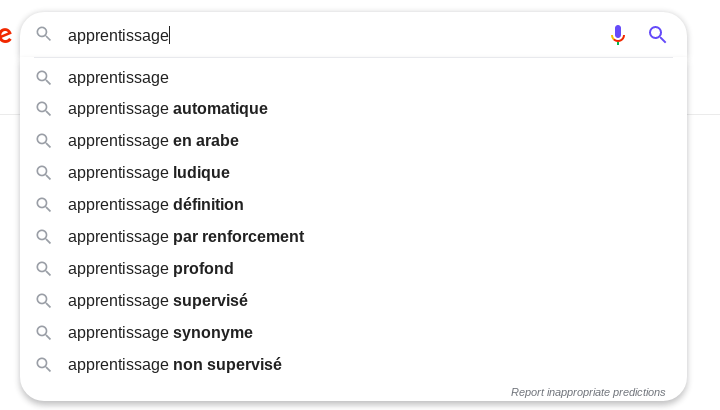
\includegraphics[height=.87\textheight]{..//img/Bweb02-ri-gmail/google-autocomplete.png}
\end{center}

\end{frame}

\begin{frame}
\frametitle{Rechercher avec Google: Effectuer une recherche}
\framesubtitle{Entrer une requête}
%\def\arraystretch{2}
\begin{tabular}{p{.7\textwidth}cp{.2\textwidth}}
	
	\hline
	
	 
\includegraphics[height=1cm]{..//img/Bweb02-ri-gmail/google-input-text.png} &
	& 
	Texte  \\
	
	\hline
	
	
\includegraphics[height=1cm]{..//img/Bweb02-ri-gmail/google-input-audio.png} &
	& 
	Audio \\
	
	\hline
	
	
\includegraphics[height=2.5cm]{..//img/Bweb02-ri-gmail/google-input-image.png} & 
	& 
	Image \\
	
	\hline

\end{tabular}

\end{frame}

\begin{frame}
\frametitle{Rechercher avec Google: Effectuer une recherche}
\framesubtitle{Services}

En plus de la recherche normale, Google offre d'autres services de recherche: 
\begin{itemize}
	\item Actualités
	\item Images
	\item Vidéos
	\item Maps
\end{itemize}

\end{frame}

\begin{frame}
\frametitle{Rechercher avec Google: Effectuer une recherche}
\framesubtitle{Services: Actualités}

\begin{center}
	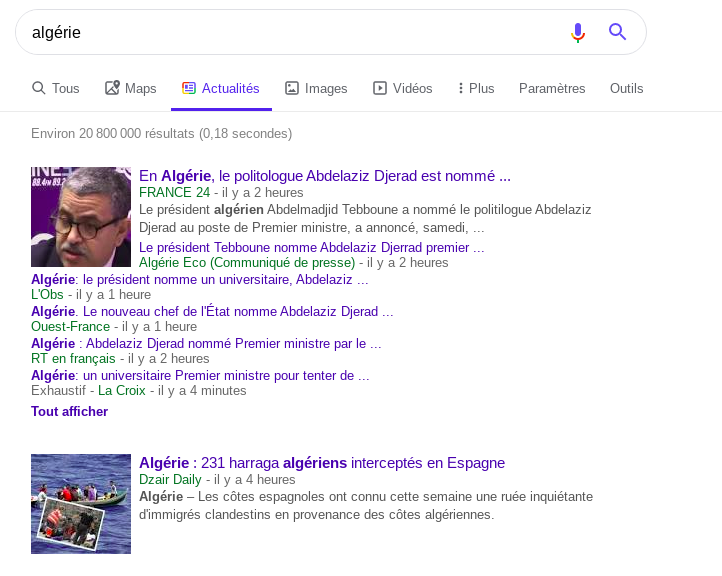
\includegraphics[height=.87\textheight]{..//img/Bweb02-ri-gmail/google-news.png}
\end{center}

\end{frame}

\begin{frame}
\frametitle{Rechercher avec Google: Effectuer une recherche}
\framesubtitle{Services: Images}

\begin{center}
	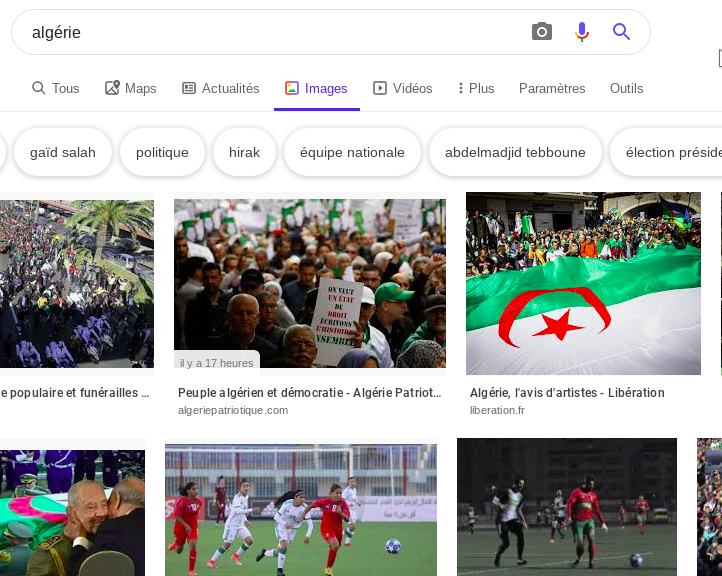
\includegraphics[height=.87\textheight]{..//img/Bweb02-ri-gmail/google-images.png}
\end{center}

\end{frame}

\begin{frame}
\frametitle{Rechercher avec Google: Effectuer une recherche}
\framesubtitle{Services: Vidéos}

\begin{center}
	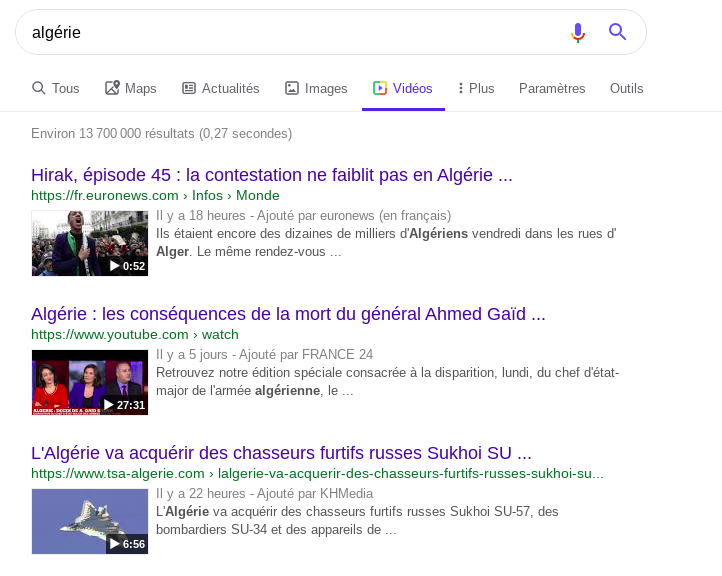
\includegraphics[height=.87\textheight]{..//img/Bweb02-ri-gmail/google-videos.png}
\end{center}

\end{frame}

\begin{frame}
\frametitle{Rechercher avec Google: Effectuer une recherche}
\framesubtitle{Services: Maps}

\begin{center}
	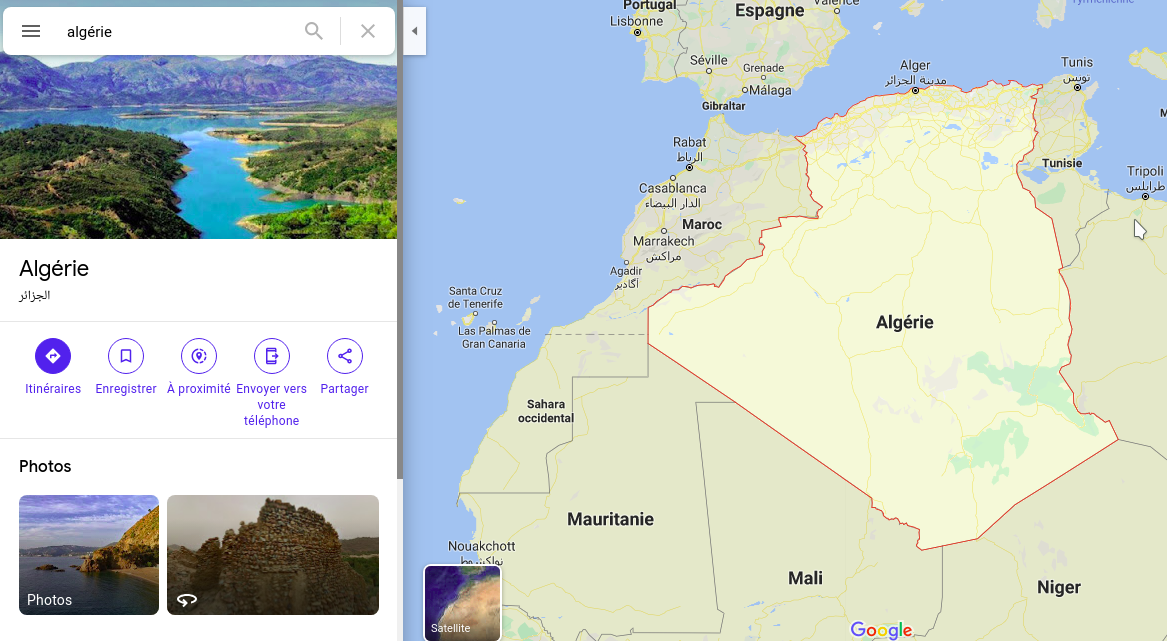
\includegraphics[height=.8\textheight]{..//img/Bweb02-ri-gmail/google-maps.png}
\end{center}

\end{frame}

\begin{frame}
\frametitle{Rechercher avec Google: Effectuer une recherche}
\framesubtitle{Les opérateurs de recherche}

% https://support.google.com/websearch/answer/2466433?hl=fr
\scriptsize\bfseries
\begin{tabular}{p{.2\textwidth}p{.25\textwidth}p{.45\textwidth}}
	
	\hline
	Opération & Exemple & Explication \\
	\hline 
	
	Rechercher plusieurs mots & université algérie & 
	Trouver les pages contenant \textcolor{red}{université} et \textcolor{red}{algérie} quelque soit l'ordre d'apparition \\
	\hline
	
	Rechercher un mot ou un autre & université \textcolor{red}{OR} algérie & 
	Trouver les pages contenant soit \textcolor{red}{université} ou \textcolor{red}{algérie} et pas les deux \\
	\hline
	
	Rechercher une correspondance exacte & \textcolor{red}{"}université en algérie\textcolor{red}{"} & 
	Trouver les pages contenant cette expression telle qu'elle est \\
	\hline
	
	Exclure des mots de votre recherche & université \textcolor{red}{-}algérie & 
	Trouver les pages contenant \textcolor{red}{université} et ne contenant pas \textcolor{red}{algérie}\\
	\hline
	
	Rechercher dans une plage de nombres & smartphone 150000\textcolor{red}{..}200000 dzd & 
	Trouver les pages contenant un nombre entre \textcolor{red}{150000} et \textcolor{red}{200000} en plus des deux autres mots\\
	\hline
	
	Rechercher un site spécifique & admis \textcolor{red}{\NoAutoSpacing site:}esi.dz & 
	Trouver les pages contenant \textcolor{red}{admis} dans le site web \textcolor{red}{esi.dz} \\
	\hline
	
	Rechercher un format spécifique & réseaux \textcolor{red}{\NoAutoSpacing filetype:}pdf & 
	Trouver les fichiers pdf contenant le mot \textcolor{red}{réseaux}\\
	\hline
	
	
\end{tabular}


\end{frame}


\subsection{Paramètres et outils de recherche}

\begin{frame}
\frametitle{Rechercher avec Google}
\framesubtitle{Paramètres et outils de recherche}

\begin{center}
	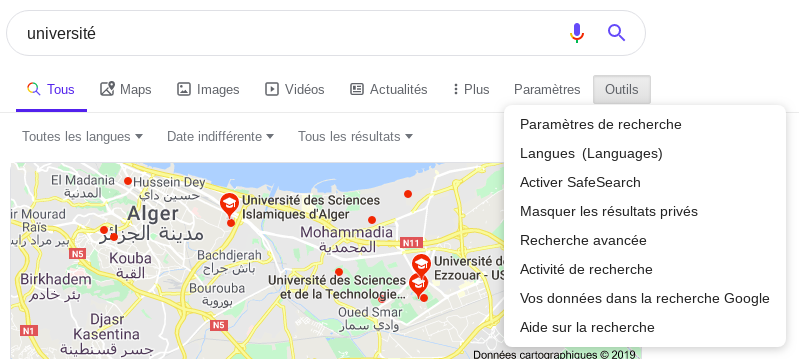
\includegraphics[width=\textwidth]{..//img/Bweb02-ri-gmail/google-param-outil.png}
\end{center}

\end{frame}

\begin{frame}
\frametitle{Rechercher avec Google: Paramètres et outils}
\framesubtitle{Paramètres: Langue}

\begin{center}
	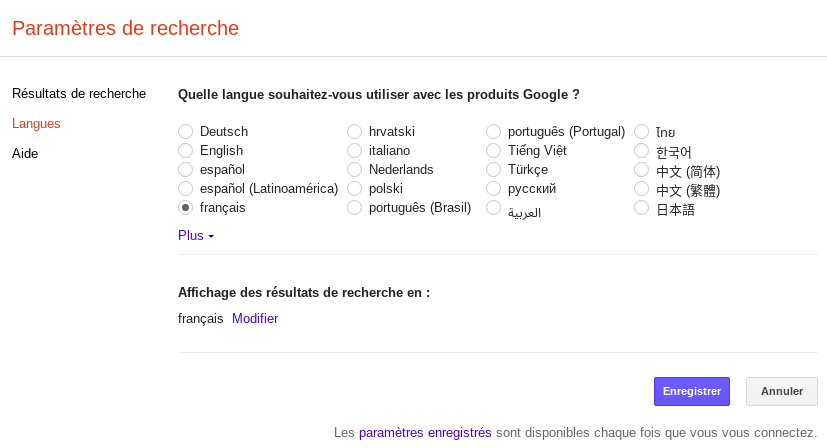
\includegraphics[height=.87\textheight]{..//img/Bweb02-ri-gmail/google-param-lang.png}
\end{center}

\end{frame}

\begin{frame}
\frametitle{Rechercher avec Google: Paramètres et outils}
\framesubtitle{Paramètres: Recherche avancée}

\begin{center}
	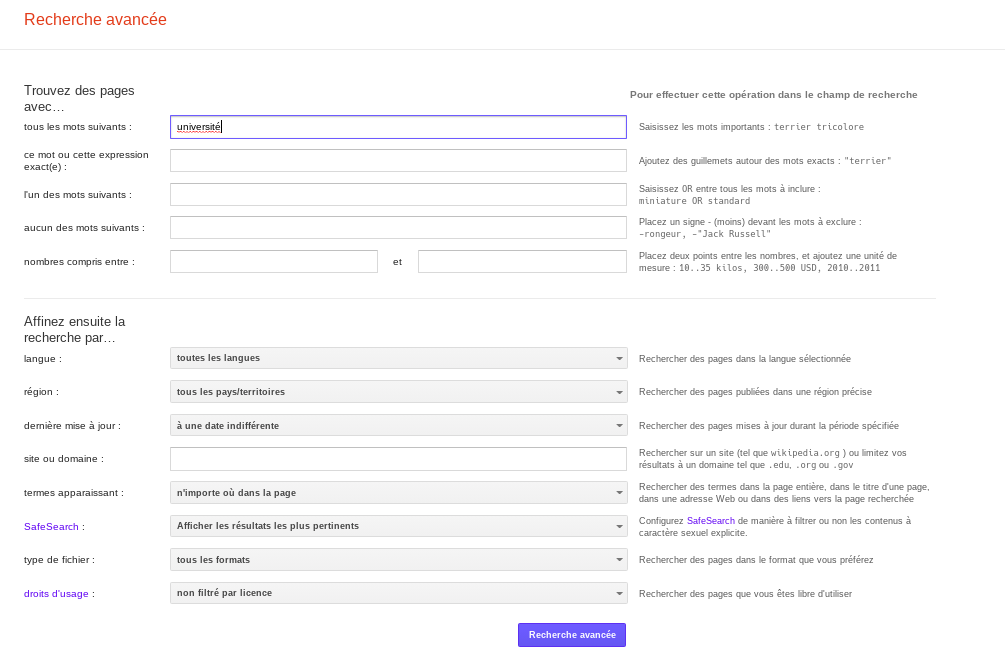
\includegraphics[height=.87\textheight]{..//img/Bweb02-ri-gmail/google-param-avance.png}
\end{center}

\end{frame}

\begin{frame}
\frametitle{Rechercher avec Google: Paramètres et outils}
\framesubtitle{Paramètres: Activité de recherche}

\begin{center}
	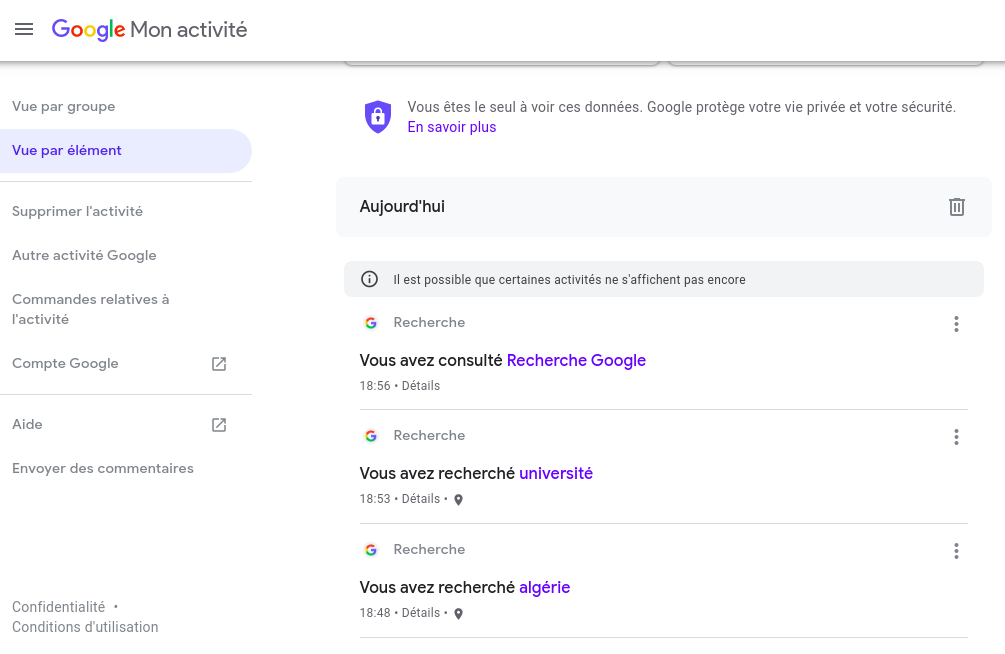
\includegraphics[height=.87\textheight]{..//img/Bweb02-ri-gmail/google-param-activite.png}
\end{center}

\end{frame}

\begin{frame}
\frametitle{Rechercher avec Google: Paramètres et outils}
\framesubtitle{Outils}

\begin{tabular}{llll}
	
	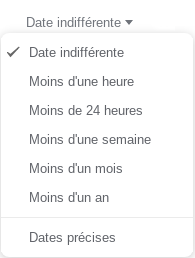
\includegraphics[width=2cm]{..//img/Bweb02-ri-gmail/google-outils-date.png} &
	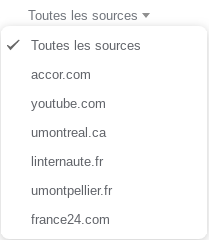
\includegraphics[width=2cm]{..//img/Bweb02-ri-gmail/google-outils-source.png} &
	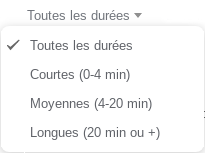
\includegraphics[width=2cm]{..//img/Bweb02-ri-gmail/google-outils-duree.png} &
	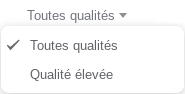
\includegraphics[width=2cm]{..//img/Bweb02-ri-gmail/google-outils-qualite.png} \\
	
	Tous &
	Vidéos &
	Vidéos &
	Vidéos \\
	
	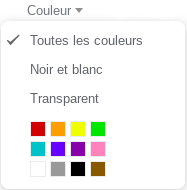
\includegraphics[width=2cm]{..//img/Bweb02-ri-gmail/google-outils-couleur.png} &
	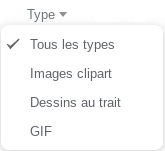
\includegraphics[width=2cm]{..//img/Bweb02-ri-gmail/google-outils-type.png} &
	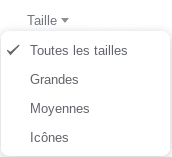
\includegraphics[width=2cm]{..//img/Bweb02-ri-gmail/google-outils-taille.png} &
	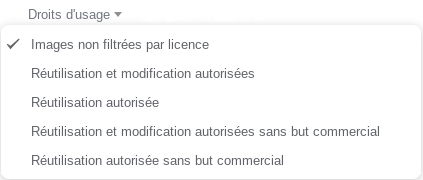
\includegraphics[width=4cm]{..//img/Bweb02-ri-gmail/google-outils-droit.png} \\
	
	Images &
	Images &
	Images &
	Images \\
	
\end{tabular}

\end{frame}

\subsection{Réponses rapides}

\begin{frame}
\frametitle{Rechercher avec Google}
\framesubtitle{Réponses rapides}

En plus de la recherche, Google offre des réponses rapides:
\begin{itemize}
	\item Calculatrice 
	\item Convertisseur d'unités
	\item Météo 
	\item Sport
	\item Dictionnaire
\end{itemize}

\end{frame}

\begin{frame}
\frametitle{Rechercher avec Google: Réponses rapides}
\framesubtitle{Calculatrice}

\begin{center}
	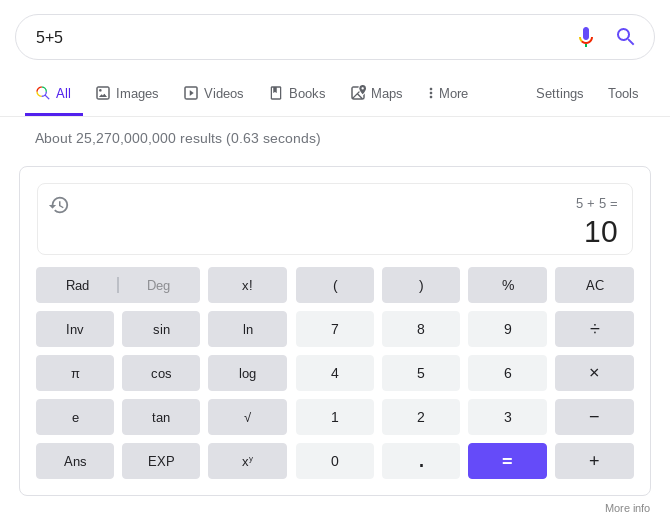
\includegraphics[height=.87\textheight]{..//img/Bweb02-ri-gmail/google-calc.png}
\end{center}

\end{frame}

\begin{frame}
\frametitle{Rechercher avec Google: Réponses rapides}
\framesubtitle{Convertisseur d'unités (ex. devises)}

\begin{center}
	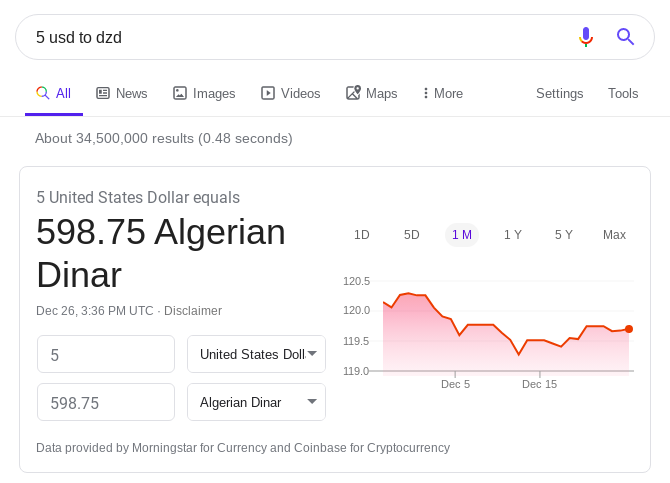
\includegraphics[height=.87\textheight]{..//img/Bweb02-ri-gmail/google-money.png}
\end{center}

\end{frame}

\begin{frame}
\frametitle{Rechercher avec Google: Réponses rapides}
\framesubtitle{Météo}

\begin{center}
	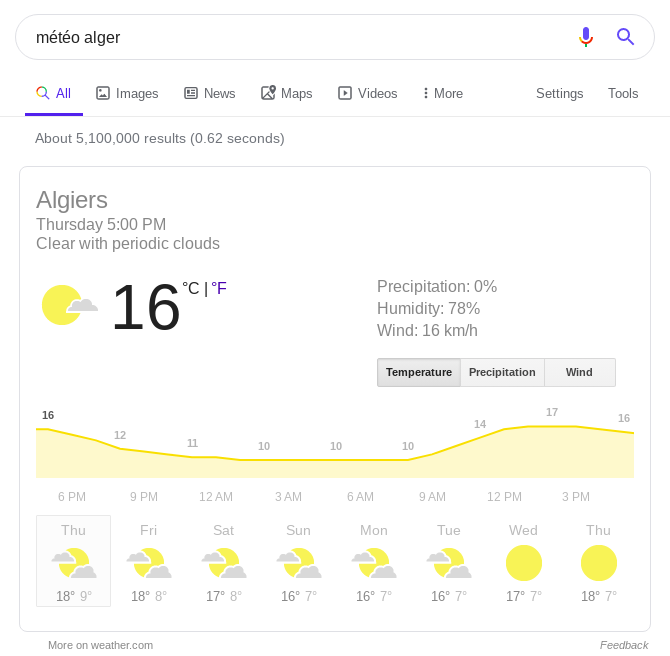
\includegraphics[height=.87\textheight]{..//img/Bweb02-ri-gmail/google-weather.png}
\end{center}

\end{frame}

\begin{frame}
\frametitle{Rechercher avec Google: Réponses rapides}
\framesubtitle{Sport}

\begin{center}
	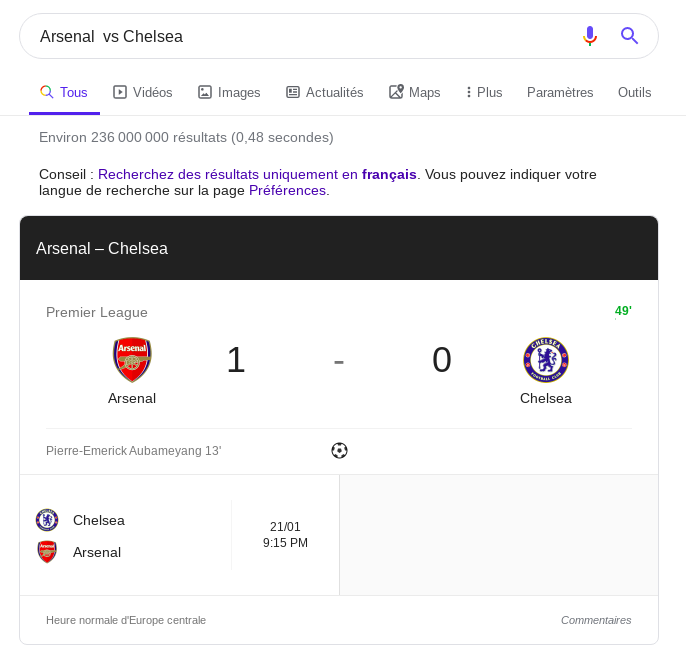
\includegraphics[height=.87\textheight]{..//img/Bweb02-ri-gmail/google-sport.png}
\end{center}

\end{frame}

\begin{frame}
\frametitle{Rechercher avec Google: Réponses rapides}
\framesubtitle{Dictionnaire}

\begin{center}
	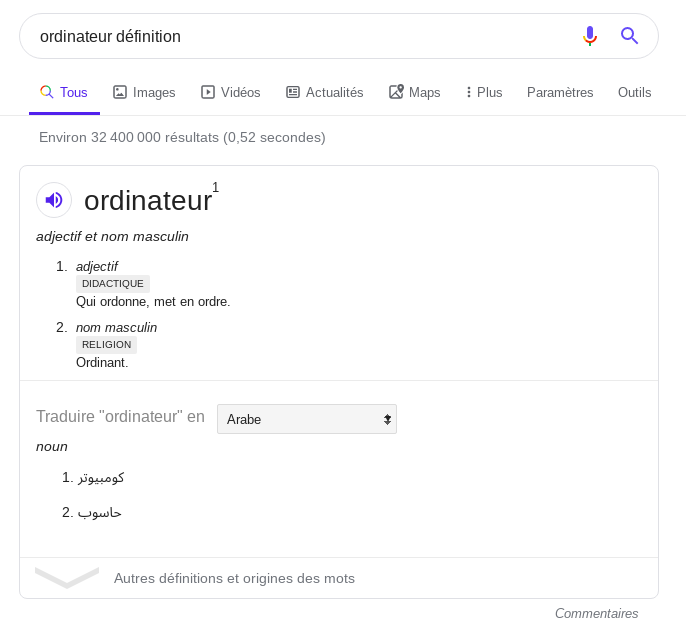
\includegraphics[height=.87\textheight]{..//img/Bweb02-ri-gmail/google-definition.png}
\end{center}

\end{frame}


%===================================================================================
\section{Messagerie électronique}
%===================================================================================

\begin{frame}
\frametitle{Messagerie électronique}

\begin{center}
	\includegraphics[height=.87\textheight]{..//img/Bweb02-ri-gmail/mail.pdf}
\end{center}

\end{frame}

\begin{frame}
\frametitle{Messagerie électronique}
\framesubtitle{Aspect légal en Algérie}


\begin{block}{Article 323 du code civil}
	L'écrit sous forme électronique est admis en tant que preuve au même titre que l'écrit sur support papier, à la condition que puisse être dûment identifiée la personne dont il émane et qu’il soit établi et conservé dans des conditions de nature à en garantir l'intégrité.
\end{block}

Un message électronique est une preuve, si on peut prouver: 
\begin{itemize}
	\item l'identité de l'expéditeur 
	\item l'intégrité du message: qu'il n'a pas été modifié 
\end{itemize} 

\end{frame}

\subsection{Accès à la messagerie}

\begin{frame}
\frametitle{Messagerie électronique}
\framesubtitle{Accès à la messagerie}

Pour accéder à la messagerie électronique, il faut avoir:
\begin{itemize}
	\item accès à l'internet
	\item un compte dans un service de messagerie.  
	\begin{itemize}
		\item On va avoir une adresse de messagerie.
		\item L'adresse se compose de deux parties séparée par @
		\item \textcolor{red}{nom-de-l'utilisateur}@\textcolor{red}{nom-de-domaine}
	\end{itemize}
	\item un moyen pour ouvrir le compte
	\begin{itemize}
		\item Navigateur web
		\item Client de messagerie 
	\end{itemize}
\end{itemize}

\end{frame}


\begin{frame}
\frametitle{Messagerie électronique: Accès à la messagerie}
\framesubtitle{Quelques services de messagerie web}

\begin{tabular}{L{.3\textwidth}{1cm}cp{.6\textwidth}}%p{.3\textwidth}
	
	\hline
	
	
\includegraphics[height=.6cm]{..//img/Bweb02-ri-gmail/gmail-logo.png} &
	&
	Gmail \\
	
	\hline
	
	
\includegraphics[height=1cm]{..//img/Bweb02-ri-gmail/outlook-logo.png} &
	& 
	Outlook.com (Hotmail, Live)  \\
	
	\hline
	
	
\includegraphics[height=.7cm]{..//img/Bweb02-ri-gmail/yahoomail-logo.png} &
	& 
	Yahoo mail \\
	
	\hline
	
	
\includegraphics[height=.7cm]{..//img/Bweb02-ri-gmail/mailcom-logo.jpg} & 
	& 
	Mail.com \\
	
	\hline
	
\end{tabular}

\end{frame}

\begin{frame}
\frametitle{Messagerie électronique: Accès à la messagerie}
\framesubtitle{Accès via le service WebMail}

\begin{wrapfigure}{r}{0.61\textwidth}
	\vspace{-1cm}
	\includegraphics[width=.60\textwidth]{..//img/Bweb02-ri-gmail/webmail.png}
	\vspace{-1cm}
\end{wrapfigure}

%Pour accéder à la messagerie électronique:

\mysphere utiliser n'importe quelle machine

\mysphere se connecter à l'internet

\mysphere ouvrir un navigateur: Google Chrome, Mozilla Firefox, Microsoft Edge, etc.  

\mysphere accéder en utilisant l'adresse webMail de votre fournisseur. 
Par exemple: \textcolor{red}{https://mail.google.com}

\mysphere n'oublier pas de fermer le compte si la machine n'est pas la votre


%\begin{itemize}
%	\item utiliser n'importe quel machine
%	\item se connecter à l'internet
%	\item ouvrir un navigateur: Google Chrome, Mozilla Firefox, Microsoft Edge, etc.  
%	\item accéder en utilisant l'adresse webMail de votre fournisseur. 
%	Par exemple: \textcolor{red}{https://mail.google.com}
%	\item n'oublier pas de fermer le compte si la machine n'est pas la votre
%\end{itemize}




\end{frame}

\begin{frame}
\frametitle{Messagerie électronique: Accès à la messagerie}
\framesubtitle{Accès via un client de messagerie}

\begin{wrapfigure}{r}{0.61\textwidth}
	\vspace{-1cm}
	\includegraphics[width=.60\textwidth]{..//img/Bweb02-ri-gmail/thunderbird4.png}
%	\vspace{-1cm}
\end{wrapfigure}

\mysphere utiliser votre machine

\mysphere installer un client de messagerie. Exemple: Mozilla Thunderbird, Microsoft Outlook (Bureau), Gmail pour Andoid (Mobile)

\mysphere Ajouter un nouveau compte et suivre les instructions 

%Pour accéder à la messagerie électronique:
%\begin{itemize}
%	\item utiliser votre machine
%	\item installer un client de messagerie. Exemple: Mozilla Thunderbird, Microsoft Outlook (Bureau), Gmail pour Andoid (Mobile).
%	\item Ajouter un nouveau compte et suivre les instructions  
%\end{itemize}

\end{frame}

\begin{frame}
\frametitle{Messagerie électronique: Accès à la messagerie}
\framesubtitle{Comparaison}

\begin{tabular}{p{.08\textwidth}p{.41\textwidth}p{.41\textwidth}}
	\hline\hline
	& Navigateur web & Client de messagerie \\
	\hline\hline
	
	Gain &
	+  
	
	+ 
	
	& 
	+ 
	
	+ 
	\\
	
	\hline
	Perte &
	- 
	
	- 
	&
	- 
	
	- 
	\\
	\hline\hline
\end{tabular}

\end{frame}

\subsection{Envoyer un message}

\begin{frame}
\frametitle{Messagerie électronique}
\framesubtitle{Envoyer un message}

Lorsqu'on veut envoyer un message, il contient les éléments suivants: 
\begin{itemize}
	\item les adresses de destinataires 
	\item l'objet du message (facultatif, mais important)
	\item le contenu et parfois des attachements
\end{itemize}

Ce message peut être localisé dans les dossiers suivants:
\begin{itemize}
	\item \textcolor{red}{Brouillon}: contient, temporairement, les messages en cours de rédaction.
	\item \textcolor{red}{Massages envoyés}: contient les messages envoyés
	\item \textcolor{red}{Corbeille}: contient les messages supprimés.
\end{itemize}

\end{frame}

\begin{frame}
\frametitle{Messagerie électronique: Envoyer un message}
\framesubtitle{Types de destinataires}

\begin{itemize}
	\item \textcolor{red}{A}: Destinataires principaux
	\begin{itemize}
		\item ceux concernés directement par le message 
		\item visible par tous les destinataires
	\end{itemize}

	\item \textcolor{red}{CC}: Copie carbone
	\begin{itemize}
		\item ceux qu'on veut informer par ce message 
		\item visible par tous les destinataires
		\item Exemple: envoyer les notes aux étudiants en utilisant le champ "A", et informer l'administration en utilisant le champ "CC".
	\end{itemize}

	\item \textcolor{red}{CCi}: Copie carbone invisible
	\begin{itemize}
		\item ceux qu'on veut cacher l'identité 
		\item non visible par les autres destinataires
		\item utile pour protéger le carnet d'adresses: personne ne peut savoir la liste de vos contactes
	\end{itemize}

\end{itemize}


\end{frame}

\begin{frame}
\frametitle{Messagerie électronique: Envoyer un message}
\framesubtitle{Objet et contenu d'un message}

\begin{itemize}
	\item \textcolor{red}{Objet}: Si vous voulez qu'on vous prend au sérieux
	\begin{itemize}
		\item on doit fournir un objet (même s'il n'est pas obligatoire)
		\item il doit être clair et court 
	\end{itemize}
	
	\item \textcolor{red}{Contenu}: Il faut fournir un contenu et pas seulement un objet long 
	\begin{itemize}
		\item salutation: Bonjour, Bonsoir, etc.
		\item se présenter, si le destinataire ne vous connait pas. 
		\item le message: il doit être clair, regroupé en paragraphes s'il est long et lisible (utiliser les puces, les numérotations, les couleurs, etc.)
		\item formule de politesse: Cordialement, Respectueusement, etc.
	\end{itemize}
	
	\item \textcolor{red}{Pièce jointe}: pas obligatoire, mais utile 
	\begin{itemize}
		\item appelé, aussi, attachement
		\item transmettre des documents
	\end{itemize}
	
\end{itemize}

\end{frame}

\begin{frame}
\frametitle{Messagerie électronique: Envoyer un message}
\framesubtitle{Signature}

\begin{itemize}
	\item lorsqu'on envoie un message, on est toujours obligé de se présenter 
	\item la solution est d'utiliser une signature 
	\item à chaque fois qu'on écrive un message, la signature sera insérée automatiquement à la fin de ce message
	\item elle peut être utilisée, aussi, pour faire de la publicité à votre site, votre blog et les différentes moyennes de contacte
\end{itemize}


\end{frame}

%\begin{frame}
%\frametitle{Messagerie électronique: Envoyer un message}
%\framesubtitle{Gestion de contactes}
%
%
%\end{frame}


\subsection{Recevoir un message}

\begin{frame}
\frametitle{Messagerie électronique}
\framesubtitle{Recevoir un message}


\end{frame}

\begin{frame}
\frametitle{Messagerie électronique: Recevoir un message}
\framesubtitle{Les informations}

De: 

A/CC/CCi

Date 

Objet


\end{frame}

\begin{frame}
\frametitle{Messagerie électronique: Recevoir un message}
\framesubtitle{Les actions}




\end{frame}

\begin{frame}
\frametitle{Messagerie électronique: Recevoir un message}
\framesubtitle{Filtrage de messages}

Spam

Virus 

Fishing 


\end{frame}


%===================================================================================
\section{Messagerie Gmail}
%===================================================================================

\begin{frame}
\frametitle{Messagerie Gmail}

\end{frame}


\begin{frame}
\frametitle{Références}

\tiny

\begin{itemize}
	\item Felix Naumann (2011). 
	"\textit{Chapter 2 – Architecture}". 
	Search Engines. 
	Universität Potsdam, Allemagne. Présentation.
	\url{https://hpi.de/fileadmin/user_upload/fachgebiete/naumann/folien/SS11/Search_Engines/SearchEngines_02_Architecture.pdf}
	
	\item Raghu Ramakrishnan (date-indéfinie).
	"\textit{Chapter 27: Information Retrieval and XML Data Management (Web search engines}". 
	Database Management Systems. 
	University of Wisconsin-Madison, Etats unis. Présentation.
	\url{http://pages.cs.wisc.edu/~dbbook/openAccess/thirdEdition/slides/slides3ed-english/Ch27c_ir3-websearch-95.pdf}
	
	\item \url{https://support.google.com/websearch/answer/134479?hl=fr}
	
\end{itemize}

\end{frame}

%\subsection{Bibliography}
%\frame[allowframebreaks]%
%{\frametitle{Bibliography}
%\tiny
%\bibliography{biblio}
%\bibliographystyle{apalike} 
%}


\end{document}

